\documentclass[11pt,oneside]{article}
\usepackage[utf8]{inputenc}
\usepackage[a4paper,top=2cm,left=2cm,right=2cm,bottom=2cm]{geometry}
\usepackage{import}
\usepackage[T1]{fontenc}
\usepackage[german,ngerman]{babel}
\usepackage[table]{xcolor}
\usepackage{amsthm, esvect}
\usepackage{mathtools}
\RequirePackage{amssymb, amsfonts, amsmath, latexsym, verbatim, xspace}
\usepackage{systeme}
\usepackage{multicol}
\usepackage{multirow}
\usepackage{framed}
\usepackage{array}
\usepackage{ragged2e}
\usepackage{graphicx}
\usepackage{pdflscape}
\usepackage{epstopdf}
\usepackage{booktabs}
\usepackage{pdfpages}
\usepackage{float} % Allows putting an [H] in \begin{figure} to specify the exact location of the figure
\usepackage{wrapfig} % Allows in-line images such as the example fish picture
\usepackage{tikz, graphicx} % tikz
\usepackage[position=top]{subfig}
\usepackage[bookmarks=true]{hyperref}%Links
\usepackage{enumerate}
\usepackage{enumitem}
\usepackage[german,ruled,vlined,linesnumbered,algosection]{algorithm2e}
\usepackage[labelfont=sf]{caption}
\usepackage{lmodern}
\usepackage{lscape}
\usepackage{tabularx}
\usepackage{systeme}
\usepackage{hhline}
\usepackage{subfiles}
\usepackage{stackengine}
\usepackage{setspace}
\usepackage{MnSymbol}
\usepackage{tcolorbox}
\usepackage{bbm}
\usepackage{url}
\usepackage{xparse}
\usepackage{sectsty}
\usepackage{array}
\usepackage{ragged2e}
\usepackage{listings} %Stellt Code-Snippets sauber dar

% definiert die Sprache
\selectlanguage{German}

% add command for different dates in Swiss fashion
\newcommand{\monthwordlong}[1]{\ifcase#1 \or Januar\or Februar\or März\or April\or Mai\or Juni\or Juli\or August\or September\or Oktober\or November\or Dezember\fi}
\newcommand{\monthwordshort}[1]{\ifcase#1\or Jan\or Feb\or Mar\or Apr\or Mai\or Jun\or Jul\or Aug\or Sept\or Okt\or Nov\or Dez\fi}
\newcommand{\datelong}{\number\day.\:\monthwordlong{\the\month}\:\number\year}
\newcommand{\dateshort}{\number\day.\:\monthwordshort{\the\month}\:\number\year}

% define color of links inside a text
\definecolor{linkblue}{RGB}{0, 0, 80}
\definecolor{plotblue}{RGB}{100, 100, 255}
\definecolor{myblue}{RGB}{8,164,214}
\definecolor{myred}{RGB}{143,42,41}
\definecolor{forestgreen}{RGB}{34,139,34}
\definecolor{highdive}{RGB}{10,169,194}
\definecolor{charcoal}{RGB}{74,74,74}
\hypersetup{
	colorlinks=true,
	linkcolor=linkblue,
	filecolor=magenta,
	urlcolor=plotblue,
	citecolor=linkblue,
	pdfpagemode=FullScreen,
}


\lstdefinestyle{mystyle}{ % definiert den style des Code-Snippets
	%backgroundcolor=\color{backcolour},
	%commentstyle=\color{codegreen},
	%keywordstyle=\color{magenta},
	%numberstyle=\tiny\color{codegray},
	%stringstyle=\color{codepurple},
	basicstyle=\ttfamily\footnotesize,
	breakatwhitespace=false,
	breaklines=true,
	captionpos=b,
	keepspaces=true,
	%numbers=left,
	%numbersep=5pt,
	showspaces=false,
	showstringspaces=false,
	showtabs=false,
	tabsize=4
}
\lstset{style=mystyle}
\usepackage{fancyhdr}

\tcbuselibrary{breakable,skins}
\usetikzlibrary{mindmap,trees}
\newlength\tindent
\setlength{\tindent}{\parindent}
\setlength{\parindent}{0pt}
\renewcommand{\indent}{\hspace*{\tindent}}

\makeatletter
\def\ifEmpty#1{\def\@temp{#1}\ifx\@temp\@empty}
\makeatother

\sectionfont{\underline}
\usetikzlibrary{arrows, petri, topaths, graphs}


% =================== BEISPIEL ====================
\theoremstyle{definition}
\newtheorem{beispiel}{Beispiel}
\renewcommand{\thebeispiel}{\arabic{beispiel}}

% =================== AUFGABE =====================
\newcounter{aufg}[section] % Zähler für die Umgebungen

\newenvironment{aufgabe}[1][]{%
    \refstepcounter{aufg}% Inkrementiere den Zähler
    \begin{tcolorbox}[%
        enhanced,
        overlay unbroken and first={\mytitleaufg[#1]}, % Titelleiste mit Icons wird nicht über Seite gebrochen
        colframe=black,
        boxrule=0pt,
        breakable,
        top=15pt,
        before=\vskip18pt,
    ]
}{%
    \end{tcolorbox}
}

\newcommand{\mytitleaufg}[1][]{% Definiert die Titelleiste und Icons
    \node[fill=black!20,
        rounded corners,
        draw=black,
        text=black,
        line width=1pt,
        inner sep=4pt,
        anchor=west,
        xshift=12pt]
        at (frame.north west){\bfseries Aufgabe \thesection.\theaufg.\ifEmpty{#1}\else\emph{ (#1)}\fi}; % Titel, letzter Teil mit ifempty testet ob #1 leer und macht Klammern und Titel, falls Titelargument übergeben wird bzw. falls #1 leer erscheint nichts - auch keine Klammern

    \node[% Icon
        rounded corners,
        text=black,
        fill=black,
        line width=0pt,
        inner sep=3pt,
        anchor=west,
        xshift=5pt,
        % yshift=-35pt
        ]
        at (frame.north east){
\includegraphics[width=24pt]{../../../Header/Icons/aufgabeicon.png}};
}

% =================== DEFINITION ==================
\newcounter{def}[section] % Zähler für die Umgebungen

\newenvironment{definition}[1][]{%
    \refstepcounter{def}% Inkrementiere den Zähler
    \begin{tcolorbox}[%
        enhanced,
        drop shadow southeast,
        overlay unbroken and first={\mytitledef[#1]}, % Titelleiste mit Icons wird nicht über Seite gebrochen
        colback=blue!5!white,
        colframe=blue!75!black,
        boxrule=2pt,
        breakable,
        top=15pt,
        before=\vskip18pt,
    ]
}{%
    \end{tcolorbox}
}

\newcommand{\mytitledef}[1][]{% Definiert die Titelleiste und Icons
    \node[fill=blue!40!white,
        rounded corners,
        draw=black,
        text=black,
        line width=1pt,
        inner sep=4pt,
        anchor=west,
        xshift=12pt]
        at (frame.north west){\bfseries Definition \thesection.\thedef.\ifEmpty{#1}\else\emph{ (#1)}\fi}; % Titel, letzter Teil mit ifempty testet ob #1 leer und macht Klammern und Titel, falls Titelargument übergeben wird bzw. falls #1 leer erscheint nichts - auch keine Klammern

    \node[% Icon
        rounded corners,
        text=black,
        fill=black,
        line width=0pt,
        inner sep=3pt,
        anchor=west,
        xshift=5pt,
        % yshift=-35pt
        ]
        at (frame.north east){
\includegraphics[width=24pt]{../../../Header/Icons/definitionicon.png}};
}

% =================== NOTATION ====================
\newcounter{nota}[section] % Zähler für die Umgebungen

\newenvironment{notation}[1][]{%
    \refstepcounter{nota}% Inkrementiere den Zähler
    \begin{tcolorbox}[%
        enhanced,
        drop shadow southeast,
        colback=yellow!5!white,
        colframe=yellow!75!black,
        overlay unbroken and first={\mytitlenota[#1]},   % Titelleiste mit Icons wird nicht über Seite gebrochen
        boxrule=2pt,
        breakable,
        top=15pt,
        before=\vskip18pt,
    ]
}{%
    \end{tcolorbox}
}

\newcommand{\mytitlenota}[1][]{% Definiert die Titelleiste und Icons
    \node[fill=yellow!40!white,,
        rounded corners,
        draw=black,
        text=black,
        line width=1pt,
        inner sep=4pt,
        anchor=west,
        xshift=12pt]
        at (frame.north west){\bfseries Notation \thesection.\thenota.\ifEmpty{#1}\else\emph{ (#1)}\fi}; % Titel, letzter Teil mit ifempty testet ob #1 leer und macht Klammern und Titel, falls Titelargument übergeben wird bzw. falls #1 leer erscheint nichts - auch keine Klammern

    \node[% Icon
        rounded corners,
        text=black,
        fill=black,
        line width=0pt,
        inner sep=3pt,
        anchor=west,
        xshift=5pt,
        % yshift=-35pt
        ]
        at (frame.north east){
\includegraphics[width=24pt]{../../../Header/Icons/definitionicon.png}};
}

% =================== SATZ ========================
\newcounter{satz}[section]  % creates a counter and resets it after each chapter

\newenvironment{satz}[1][]{   % Hauptbox mit Satz drin
    \refstepcounter{satz}
    \begin{tcolorbox}[%
        enhanced,
        colback=red!5!white,
        fuzzy halo=2mm with gray,
        colframe=red!75!black,
        overlay unbroken and first={\mytitlesatz[#1]},   % Titelleiste mit Icons wird nicht über Seite gebrochen
        boxrule=2pt,
        breakable,
        top=15pt,
        before=\vskip18pt,
    ]
}{%
    \end{tcolorbox}
}

\newcommand{\mytitlesatz}[1][]{                     % Macht Titelbox und Icons
   \node[fill=red!90!white,
      rounded corners,
      draw=black,,
      text=black,
      line width=1pt,
      inner sep=4pt,
      anchor=west,
      xshift=12pt]
   at (frame.north west){\bfseries Satz \thesection.\thesatz.\ifEmpty{#1}\else\emph{ (#1)}\fi};  % Titel, letzter Teil mit ifx testet ob #1 leer und macht Klammern und Titel, falls Titelargument übergeben wird bzw.  falls #1 leer erscheint nichts - auch keine Klammern

 \node[ % Icon
      rounded corners,
      text=black,
      fill=black,
      line width=0pt,
      inner sep=3pt,
      anchor=west,
      xshift=5pt,
%     yshift=-35pt
]
   at (frame.north east){ 
\includegraphics[width=24pt]{../../../Header/Icons/satzicon.png} };
}

% =================== BEWEIS ======================
\newenvironment{beweis}[1][]{
    \begin{tcolorbox}[
        enhanced,
        overlay unbroken and first={\mybeweis[#1]},     % Titelleiste mit Icons wird nicht über Seite gebrochen
        colback=white,
        colframe=black,
        boxrule=0pt,
        breakable,
        top=15pt,
        before=\vskip18pt,
    ]
}{
        \end{tcolorbox}
}

\newcommand{\mybeweis}[1][]{                     % Macht Titelbox und Icons
   \node[fill=white,
      rounded corners,
      draw=black,
      text=black,
      line width=1pt,
      inner sep=4pt,
      anchor=west,
      xshift=12pt]
   at (frame.north west){\bfseries Beweis \ifEmpty{#1}\else\emph{ (#1)}\fi};  % Titel, letzter Teil mit ifx testet ob #1 leer und macht Klammern und Titel, falls Titelargument übergeben wird bzw.  falls #1 leer erscheint nichts - auch keine Klammern
}

% =================== ALGORITHM ===================
\newcounter{algo}[section]  % creates a counter and resets it after each chapter

\newenvironment{algo}[1][]{   % Hauptbox mit Satz drin
    \refstepcounter{algo}
    \begin{tcolorbox}[%
        enhanced,
        drop shadow southeast,
        colback=yellow!5!white,
        colframe=yellow!75!black,
        overlay unbroken and first={\algotitle[#1]},   % Titelleiste mit Icons wird nicht über Seite gebrochen
        boxrule=2pt,
        breakable,
        top=15pt,
        before=\vskip18pt,
    ]
}{%
    \end{tcolorbox}
}

\newcommand{\algotitle}[1][]{                     % Macht Titelbox und Icons
   \node[fill=yellow!40!white,
      rounded corners,
      draw=black,
      text=black,
      line width=1pt,
      inner sep=4pt,
      anchor=west,
      xshift=12pt]
   at (frame.north west){\bfseries \ifEmpty{#1}{Ablauf}\else{#1}\fi};  % Titel, letzter Teil mit ifx testet ob #1 leer und macht Klammern und Titel, falls Titelargument übergeben wird bzw.  falls #1 leer erscheint nichts - auch keine Klammern

 \node[ % Icon
      rounded corners,
      text=black,
      fill=black,
      line width=0pt,
      inner sep=3pt,
      anchor=west,
      xshift=5pt
      % yshift=-35pt
      ]
   at (frame.north east){ 
\includegraphics[width=24pt]{../../../Header/Icons/algoicon.png} };
}

% ================ Nummerierte Multicol ================
\newenvironment{enumcols}[1][]{
    \begin{enumerate}[label=\alph*)]\begin{multicols}{#1}
}{
    \end{multicols}\end{enumerate}
}



% =================================================
\usetikzlibrary{shapes,arrows}
\tikzstyle{decision} = [diamond, draw, fill=blue!20,
    text width=6em, text badly centered, node distance=4cm, inner sep=0pt]
\tikzstyle{block} = [rectangle, draw, fill=blue!20,
    text width=8em, text centered, rounded corners, minimum height=4em]
\tikzstyle{line} = [draw, -latex']
\tikzstyle{cloud} = [draw, ellipse,fill=red!20, node distance=2cm,
    minimum height=2em]

% Karriertes Papier für Antwort
\newcommand{\karos}[1]{\begin{tikzpicture}\draw[step=0.5cm,color=gray] (0,0) grid (\linewidth,#1 cm);\end{tikzpicture}}
%%
% Header and Footer
%%
\linespread{1.2} % Line spacing
\fancypagestyle{plain}{
	\pagestyle{fancy}
	\lhead{}
	\chead{}
	\rhead{}
	\lfoot{\Autor}
	\cfoot{\Skriptname}
	\rfoot{\thepage}
	\renewcommand{\headrulewidth}{0pt}
	\renewcommand{\footrulewidth}{0.4pt}
}

\pagestyle{fancy}
\fancyhf{}
\rhead{\rightmark}
\lfoot{\leftmark}
\rfoot{\thepage}
\renewcommand{\headrulewidth}{0.2pt}
%\setlength\parindent{0pt} % Uncomment to remove all indentation from paragraphs



%%
% Math Arrows
%%
\newcommand{\same}{\ensuremath{\Longleftrightarrow}}
\renewcommand{\to}{\ensuremath{\longrightarrow}}
\newcommand{\qsame}{\quad\same\quad}
\newcommand{\dsame}{\ensuremath{:\Leftrightarrow}}
\newcommand{\qdsame}{\quad\dsame\quad}
\newcommand{\ldsame}{\ensuremath{:\Longleftrightarrow}}
\newcommand{\samedef}{\ensuremath{\us {\text{def}} \Leftrightarrow}}
\newcommand{\qsamedef}{\quad\samedef\quad}
\newcommand{\lsamedef}{\ensuremath{\us {\text{def}} \Longleftrightarrow}}
\newcommand{\qlsamedef}{\quad\lsamedef\quad}


%%
% Mengendefinitionen
%%
\newcommand{\M}{\ensuremath{\mathcal{M}}}
\newcommand{\N}{\ensuremath{\mathbb{N}}}
\newcommand{\Z}{\ensuremath{\mathbb{Z}}}
\newcommand{\Q}{\ensuremath{\mathbb{Q}}}
\newcommand{\I}{\ensuremath{\mathbb{I}}}
\newcommand{\R}{\ensuremath{\mathbb{R}}}
\newcommand{\C}{\ensuremath{\mathbb{C}}}
\renewcommand{\S}{\ensuremath{\mathbb{S}}}
\newcommand{\Prim}{\ensuremath{\mathbb{P}}}
\newcommand{\0}{\ensuremath{\emptyset}}
\renewcommand{\Re}{\ensuremath{\operatorname{Re}}}
\renewcommand{\Im}{\ensuremath{\operatorname{Im}}}
\newcommand{\strich}{\ensuremath{\big\vert}}

%%
% Mengenoperation
%%
\renewcommand{\nin}{\not\in}


%%
% Logisches Und und Oder
%%
\newcommand{\sand}{\ensuremath{\; \land \;}}
\newcommand{\sor}{\ensuremath{\; \lor \;}}
\renewcommand{\*}{\ensuremath{\cdot}}
\newcommand{\oder}{\vee}
\newcommand{\n}{\neg}
\newcommand{\und}{\wedge}


%%
% Bei Integral, Summe,... die Grenzen über bzw.
% unter das Zeichen
%%
\renewcommand{\d}[1]{\ensuremath{\operatorname{d}\!{#1}}}
\newcommand{\Sum}{\sum\limits}
\newcommand{\Prod}{\prod\limits}
\newcommand{\Min}{\min\limits}
\newcommand{\Max}{\max\limits}
\newcommand{\Lim}{\lim\limits}
\newcommand{\Inf}{\inf\limits}
\newcommand{\Sup}{\sup\limits}
\newcommand{\Liminf}{\liminf\limits}
\newcommand{\Limsup}{\limsup\limits}
%\renewcommand{\Cup}{\bigcup\limits}
%\renewcommand{\Cap}{\bigcap\limits}
\newcommand{\Otimes}{\bigotimes\limits}
\newcommand{\Oplus}{\bigoplus\limits}


%%
% Arcus Cotangens, Logarithmus
%%
\let\oldsin\sin
\renewcommand{\sin}[1]{\oldsin{\left(#1\right)}}
\let\oldcos\cos
\renewcommand{\cos}[1]{\oldcos{\left(#1\right)}}
\let\oldtan\tan
\renewcommand{\tan}[1]{\oldtan{\left(#1\right)}}
\let\oldarcsin\arcsin
\renewcommand{\arcsin}[1]{\oldarcsin{\left(#1\right)}}
\let\oldarccos\arccos
\renewcommand{\arccos}[1]{\oldarccos{\left(#1\right)}}
\let\oldarctan\arctan
\renewcommand{\arctan}[1]{\oldarctan{\left(#1\right)}}
\let\oldln\ln
\renewcommand{\ln}[1]{\oldln{\left(#1\right)}}
\newcommand{\Log}[2]{\ensuremath{\operatorname{log}_{#1}\left(#2\right)}}
\newcommand{\e}{\operatorname{e}}
\renewcommand{\exp}[1]{\ensuremath{\operatorname{\e}^{#1}}}


%%
% Griechische Buchstaben
%%
\renewcommand{\epsilon}{\ensuremath{\varepsilon}}
\renewcommand{\phi}{\varphi}
\renewcommand{\l}{\lambda}
\renewcommand{\t}{\tau}


%%
% Bezeichnungen
%%
\newcommand{\Rgn}{\R_{>0}} % R grösser Null
\newcommand{\Rad}{\operatorname{Rad}}   % Radikal
\newcommand{\kgV}{\operatorname{kgV}}   % Kleinster gemeinsame Vielfache
\newcommand{\ggT}{\operatorname{ggT}}   % Grösster gemeinsame Teiler
\newcommand{\winkel}{\sphericalangle}          % Winkelsymbol
\DeclarePairedDelimiter\abs{\lvert}{\rvert} % besserer Betrag
\makeatletter
\let\oldabs\abs
\def\abs{\@ifstar{\oldabs}{\oldabs*}}
\makeatother


%%
% Vektorgeometrie
%%
\renewcommand{\v}[1]{\vv{#1}}       % besserer Pfeil über Buchstaben
\renewcommand{\vec}[2]{\begingroup\renewcommand{\arraystretch}{1}\left(\begin{array}{c} #1 \\ #2 \end{array}\right)\endgroup}   % two dimensional vector
\renewcommand{\Vec}[3]{\begingroup\renewcommand{\arraystretch}{1}\left(\begin{array}{c} #1 \\ #2 \\ #3 \end{array}\right)\endgroup}      % three dimensional vector


%%
% Text
%%
\newcommand*{\Ueq}[1]{\mathrel{\mathop{=}\limits_{\text{#1}}}}
\newcommand*{\Oeq}[1]{\mathrel{\stackrel{\text{#1}}{=}}}
\newcommand{\utext}[2]{\underbrace{#1}_{\substack{#2}}}
\newcommand{\otext}[2]{$\overbrace{\textrm{#1}}^{\textrm{#2}}$}
\newcommand{\lineortext}[1]{\hspace{0,1cm}\underline{\hspace{0.1cm}\hphantom{#1}\hspace{0.1cm}}\hspace{0,1cm}} % Lückentext erstellen
\newcommand{\gap}[1]{\rule{#1 cm}{1pt}}
\graphicspath{{images/}}


\newcommand{\Skriptname}{Quadratische Funktionen}
\newcommand{\Autor}{Jonas Guler (Gu)}
\newcommand{\version}{\textit{v}1.0}

\begin{document}
\begin{titlepage}
	\clearpage
	\title{\Huge\textbf{\Skriptname} \\[1cm]}
	\author{Autor:\\ \Autor}
	\date{\normalsize {Version \version}\\ \datelong}
	\maketitle
	\thispagestyle{empty}
	\vfill
	\tableofcontents
\end{titlepage}
\pagenumbering{arabic}
%############################################################################################
\subsection*{Erinnerung: Was ist eine Funktion?}
	Wir haben den Begriff einer Funktion vor gut einem Jahr das erste Mal kennen gelernt. Dabei sind folgende Komponenten zentral:
	\begin{itemize}
		\item Definitionsmenge
		\item Wertemenge
		\item Zuordnungsvorschrift/Funktionsgleichung
		\item Wertetabelle
		\item Graph der Funktion
	\end{itemize}
	\begin{definition}
		Unter einer Funktion $f$ versteht man eine eindeutige Zuordnung. Dabei wird jeder Zahl $x$ aus der Definitionsmenge genau einen Wert $y$ aus der Wertemenge zugeordnet.
		\begin{figure}[H]
			\centering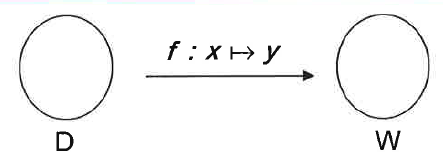
\includegraphics[scale=0.6]{RepFunktion.png}
		\end{figure}
	\end{definition}
	Eine Funktion war meistens gegeben durch eine \textbf{Funktionsgleichung} $f(x)=\ldots$ oder $f:y=\ldots$, welche diese Zuordnungsbeziehung beschreibt. Unterscheide dabei zwischen der Funktion $f$ als Zuordnungsvorschrift und den Funktionswerten $f(x)$ , die den einzelnen $x-$Werten zugeordnet werden. Systematisch besprochen haben wir bisher vor allem \textbf{lineare Funktionen}, das heisst Funktionen der Form $f(x)=mx+q$. Der Graph einer solchen linearen Funktion ist eine \textbf{Gerade} mit der Steigung $m$ und dem $y-$Achsenabschnitt $q$.

\newpage
\section{Definition der Quadratischen Funktion}
	Der Flug eines Freestyle-Snowboarders, Wasserstrahl von Brunnen aber auch die Form vieler Brücken haben ähnliches bogenförmiges Aussehen. Zu solchen Formen passen Geraden, also lineare Funktionen, nicht, sondern neue Funktionen müssen zu ihrer Beschreibung eingeführt werden. Mit Hilfe von quadratischen Funktionen gelingen häufig sehr gute Beschreibungen.
	\begin{figure}[h]
		\begin{minipage}{0.3\linewidth}
			\centering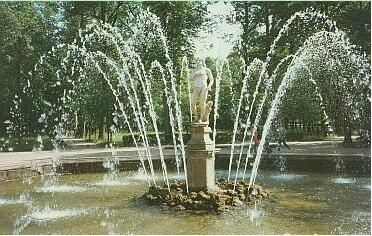
\includegraphics[width=4cm]{brunnen.png}
		\end{minipage}
		\hfill
		\begin{minipage}{0.3\linewidth}
			\centering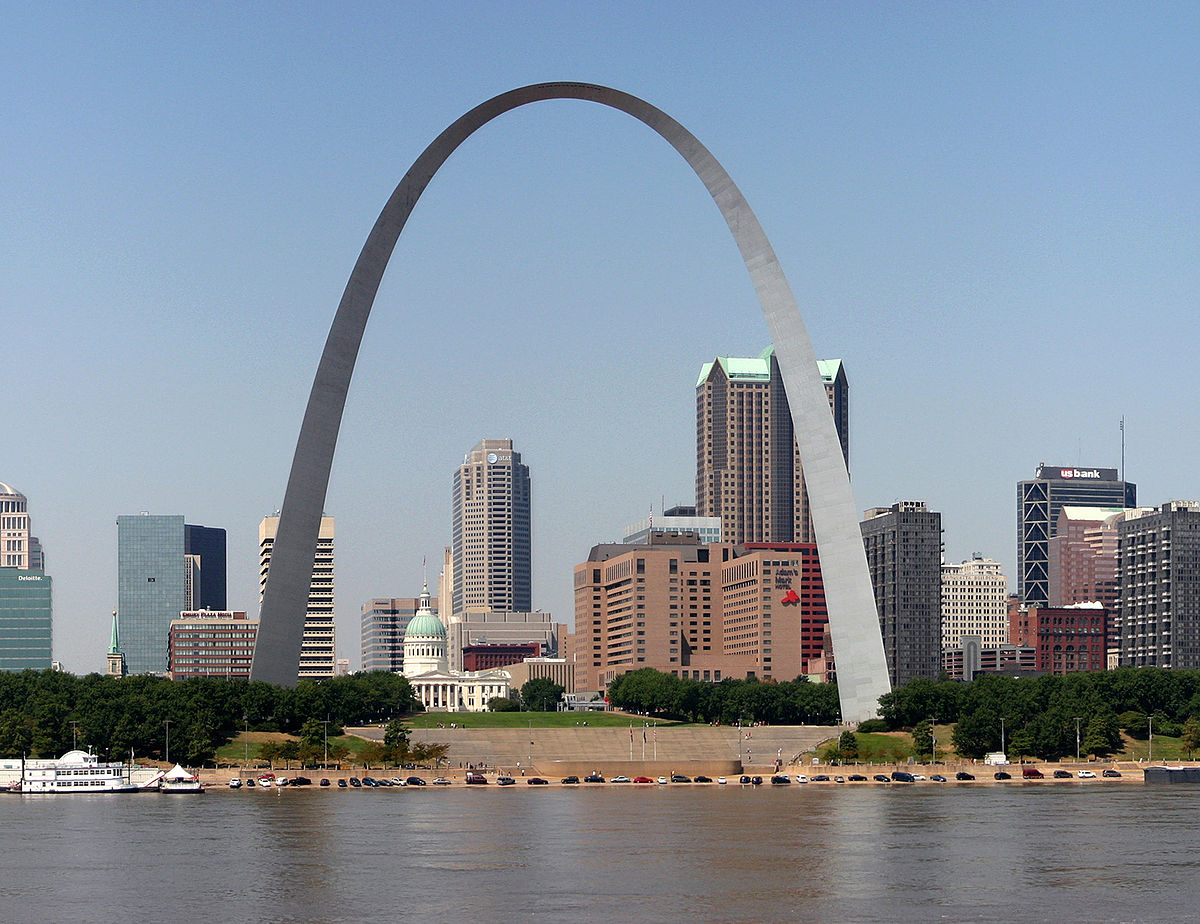
\includegraphics[width=4cm]{gatewayarch.png}
		\end{minipage}
		\hfill
		\begin{minipage}{0.3\linewidth}
			\centering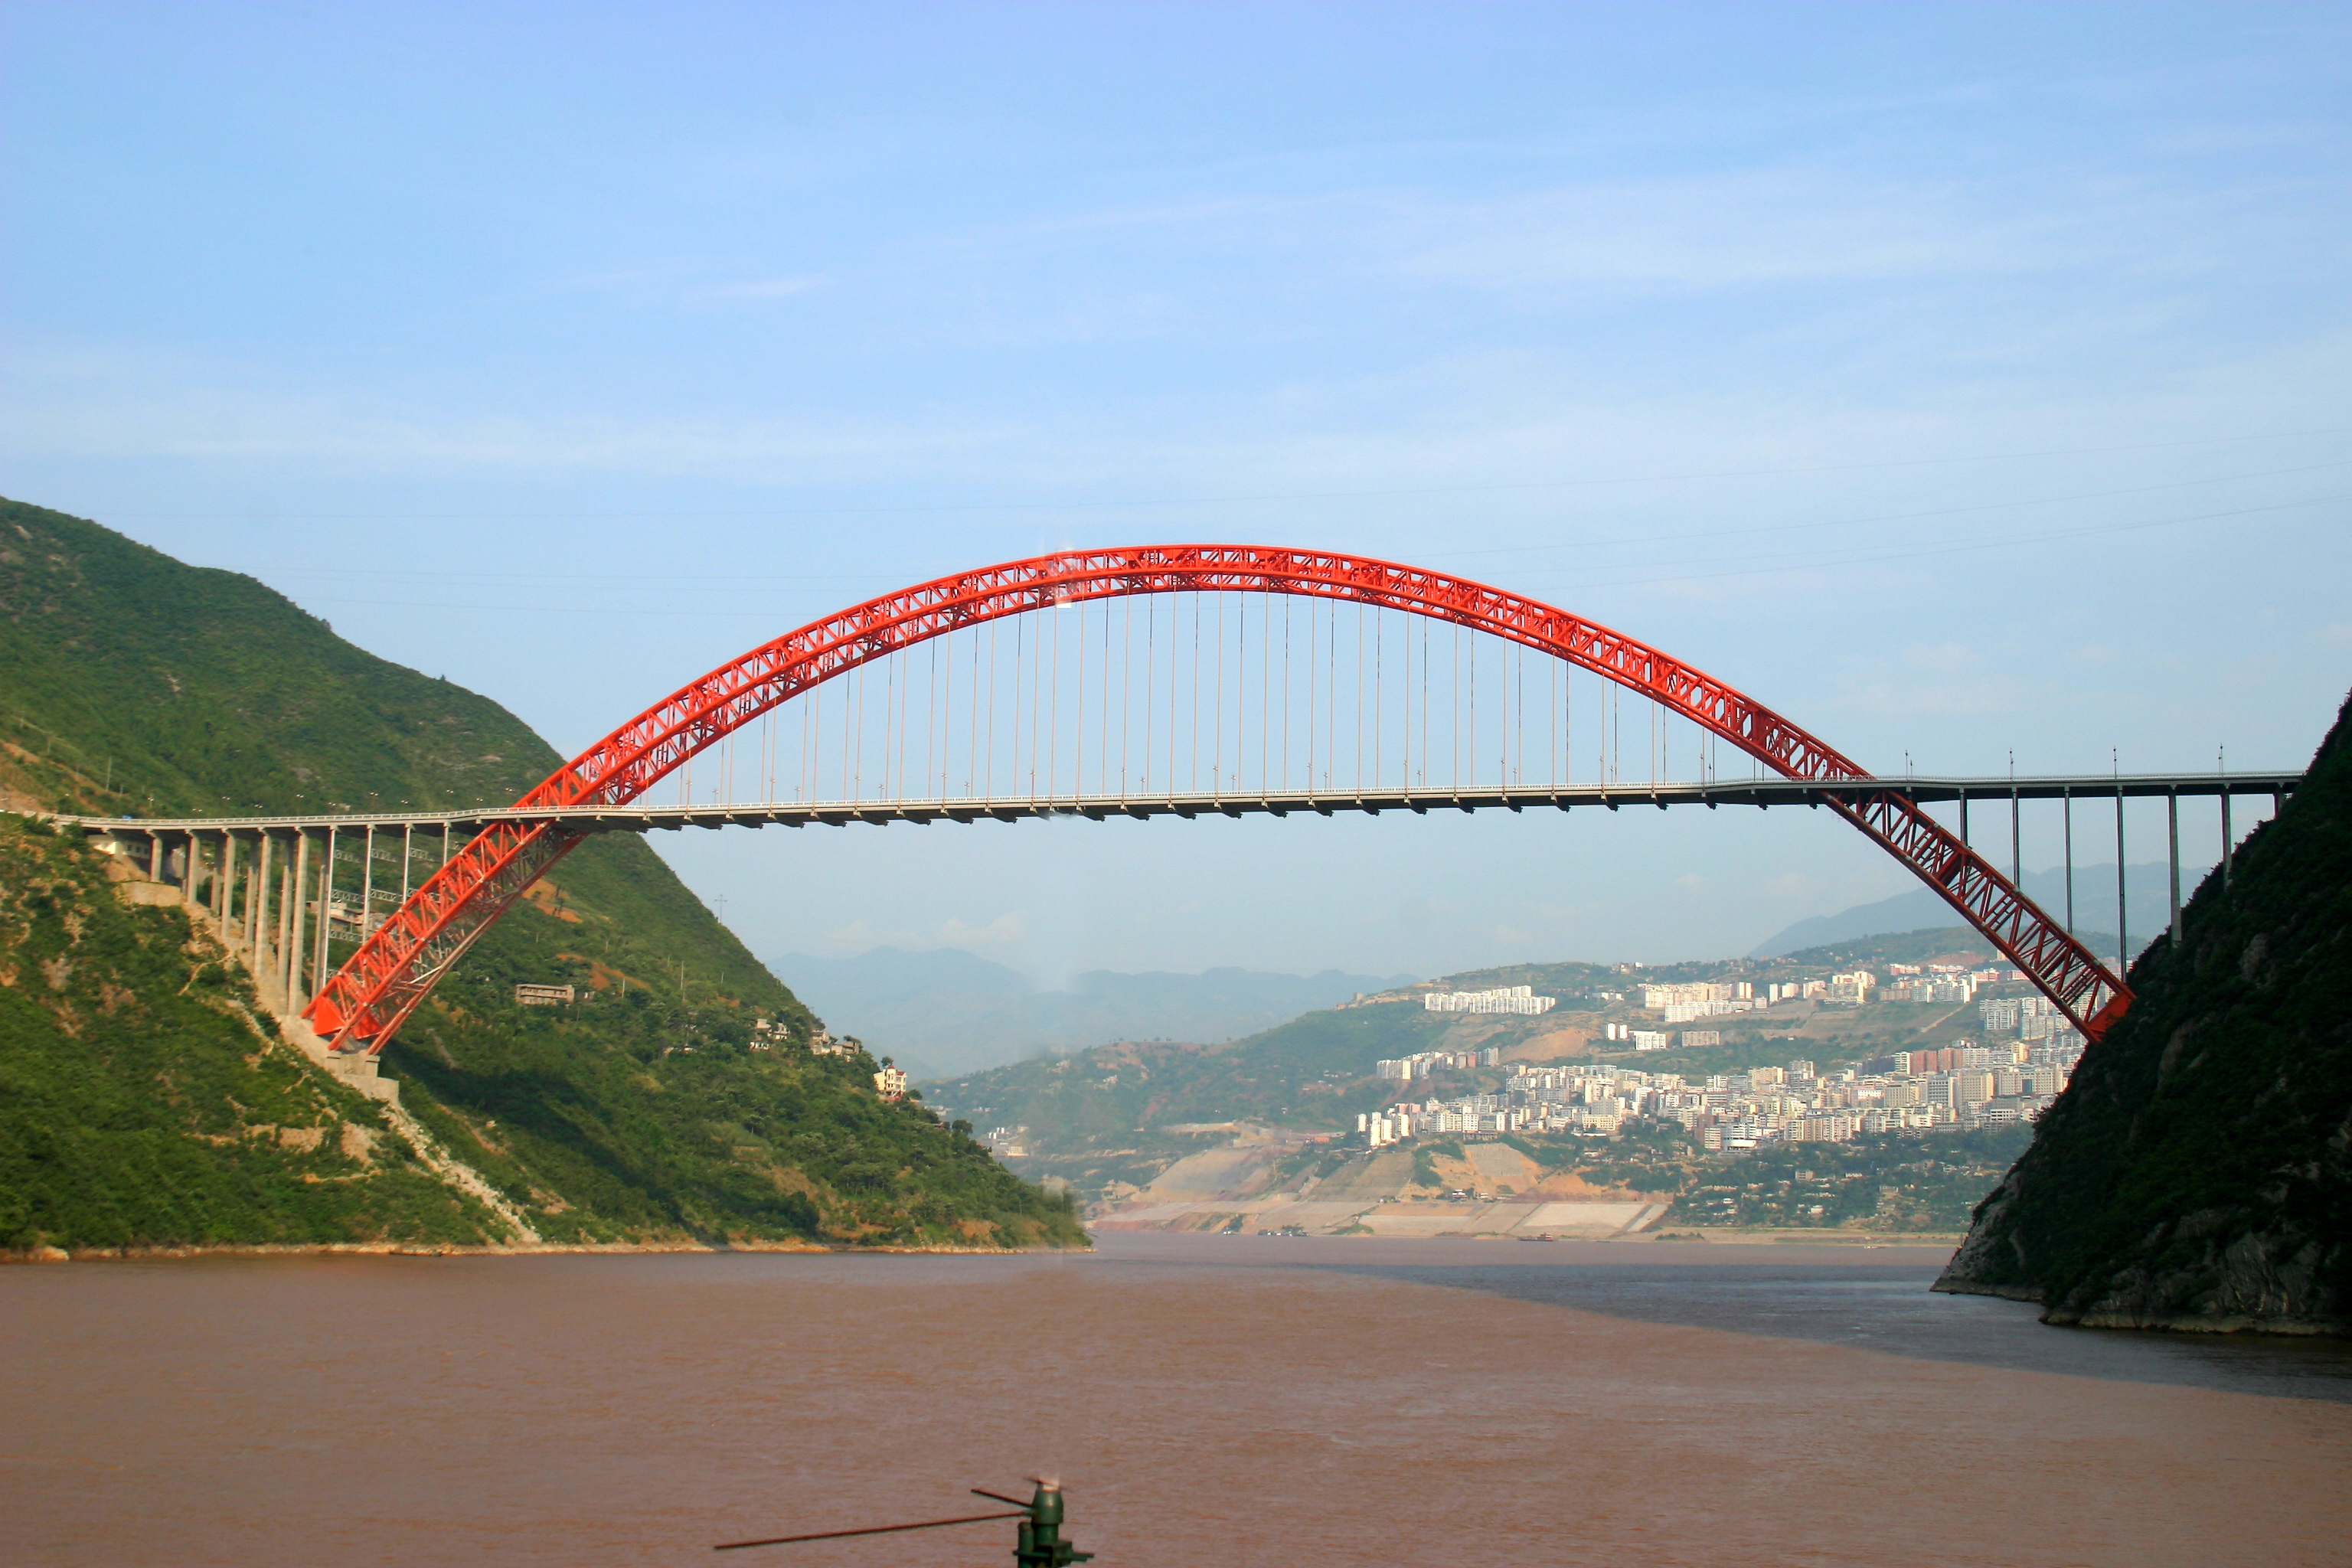
\includegraphics[width=4cm]{brücke.png}
		\end{minipage}
	\end{figure}

	Diese Funktionen treten auch in ganz anderen Zusammenhängen auf, etwa bei der Modellierung des Anhaltewegs, bei der Kalkulation von Theateraufführungen, oder der Untersuchung von Gewinnen in der Skiproduktion. Zur genaueren Berechnung von gewünschten Werten werden uns die Lösungsstrategien von quadratische Gleichungen vermehrt helfen. Bevor wir aber zu sehr ins Detail gehen, lasst uns die quadratische Gleichung zuerst mal definieren.
	\begin{definition}[Quadratische Funktionen]
		Eine Funktion, deren Funktionsgleichung in die Form \[\mathbf{f:y=ax^2+bx+c,}\] gebracht werden kann, wobei $a,b,c\in\R$ und $a\neq0$ gilt, heisst \textbf{quadratische Funktion}.\newline
		Den zugehörigen Graphen der Funktion nennt man \textbf{Parabel}.
	\end{definition}
	Ihr seht, die Ähnlichkeit zur Definition einer quadratischen Gleichung ist deutlich erkennbar. Es gibt verschiedene Formen, welche bei der Angabe einer quadratischen Funktion verwendet werden. Je nach Aufgabe bzw. Anwendung ist die eine oder andere Form sinnvoller.
	\begin{definition}
		\begin{table}[H]
			\centering
			\begin{tabular}{p{7cm} l}
				\textbf{Normalform} & $\displaystyle f:y=ax^2+bx+c$ \\
				\textbf{Scheitelpunktform} & $\displaystyle f:y=a(x-u)^2+v$ \\
				\textbf{Nullstellenform} & $\displaystyle f:y=a(x-x_1)(x-x_2)$
			\end{tabular}
		\end{table}
	\end{definition}
	\begin{aufgabe}
		Entscheide, ob die Funktionsgleichung eine lineare, quadratische Funktion oder keines von beiden beschreibt.
		\begin{enumcols}[3]
			\item $f_1(x)=4x^3-2x^2+x$
			\item $f_2(x)=3x^2+1$
			\item $f_3(x)=4x^2-2x+1-4x^2$
		\end{enumcols}
	\end{aufgabe}



\newpage
\section{Die Parabel}
	Bevor wir uns mit dem Graph einer quadratischen Funktion auseinandersetzen und dessen Eigenschaften studieren, vergleichen wir den Graph mit dem einer linearen Funktion.
	\begin{definition}
		Der Graph einer quadratischen Funktion heisst \textbf{Parabel}. Als einfachste Form nennt man den Graph von $f:y=x^2$ Normalparabel.
	\end{definition}
	\begin{aufgabe}
		\begin{enumerate}[label=\alph*)]
			\item Zeichne die Graphen der Funktionen $f:y=x^2$ und $g:y=2x+2$.\\ \emph{Erstelle zuerst eine Wertetabelle mit $-3\leq x\leq 3$, Schrittweite 0.5 und zeichne dann.}
			\begingroup
			\renewcommand{\arraystretch}{1.5}
			\begin{table}[H]
				\centering
				\begin{tabular}{|p{0.6cm}|p{0.6cm}|p{0.6cm}|p{0.6cm}|p{0.6cm}|p{0.6cm}|p{0.6cm}|p{0.6cm}|p{0.6cm}|p{0.6cm}|p{0.6cm}|p{0.6cm}|p{0.6cm}|p{0.6cm}|} \hline
					$x$  & $-3$ & $-2.5$ & $-2$ & $-1.5$ & $-1$ & $-0.5$ & $0$ & $0.5$ & $1$ & $1.5$ & $2$ & $2.5$ & $3$ \\\hline
					$f(x)$  & & & & & & & & & & & & & \\\hline
					$g(x)$  & & & & & & & & & & & & & \\\hline
				\end{tabular}
			\end{table}
			\endgroup
			\begin{minipage}{0.475\linewidth}
				\centering
				\begin{tikzpicture}[cross/.style={draw, cross out, minimum size=2*(#1-1pt), inner sep=0pt, outer sep=0pt}, x=10mm, y=10mm,
					>=latex,   %Voreinstellung für Pfeilspitzen
					font=\footnotesize, scale=0.75]
					%Raster zeichnen
					\draw [color=gray!50]  [step=5mm] (-3.4,0) grid (3.4,9.4);
					% Achsen zeichnen
					\draw[->,thick] (-3.8,0) -- (3.8,0) node[left, below] {\normalsize $x$};
					\draw[->,thick] (0,-0.8) -- (0,10) node[above, left=4pt] {\normalsize $y$};
					% Achsen beschriften
					\foreach \x in {-3,-2,-1,1,2,...,3} \draw (\x,-.1) -- (\x,.1) node[below=4pt] {$\x$};
					\foreach \y in {1,2,...,9} \draw (-.1,\y) -- (.1,\y) node[left=4pt] {$\y$};
					% Besserer Ursprung
					\draw[color=black] (0pt,-7pt) node[left] {$0$};
					%Funktionen zeichnen:
					\clip(-3.6,-0.5) rectangle (3.6,9.5); %Bildbereich
					%\draw[forestgreen,samples=100] plot (\x, \x*\x) node[above] {$f$};
					%Beschriftung
					%\node[forestgreen]  at (2.8,6.8) {\normalsize$f$};
				\end{tikzpicture}
			\end{minipage}
			\hfill
			\begin{minipage}{0.475\linewidth}
				\centering
				\begin{tikzpicture}[cross/.style={draw, cross out, minimum size=2*(#1-1pt), inner sep=0pt, outer sep=0pt}, x=10mm, y=10mm,
					>=latex,   %Voreinstellung für Pfeilspitzen
					font=\footnotesize, scale=0.75]
					%Raster zeichnen
					\draw [color=gray!50]  [step=5mm] (-3.4,0) grid (3.4,9.4);
					% Achsen zeichnen
					\draw[->,thick] (-3.8,0) -- (3.8,0) node[left, below] {\normalsize $x$};
					\draw[->,thick] (0,-0.8) -- (0,10) node[above, left=4pt] {\normalsize $y$};
					% Achsen beschriften
					\foreach \x in {-3,-2,-1,1,2,...,3} \draw (\x,-.1) -- (\x,.1) node[below=4pt] {$\x$};
					\foreach \y in {1,2,...,9} \draw (-.1,\y) -- (.1,\y) node[left=4pt] {$\y$};
					% Besserer Ursprung
					\draw[color=black] (0pt,-7pt) node[left] {$0$};
					%Funktionen zeichnen:
					\clip(-3.6,-0.5) rectangle (3.6,9.5); %Bildbereich
					%\draw[forestgreen,samples=100] plot (\x, \x*\x) node[above] {$f$};
					%Beschriftung
					%\node[forestgreen]  at (2.8,6.8) {\normalsize$f$};
				\end{tikzpicture}
			\end{minipage}
			\item Vergleiche die beiden Graphen und Tabellen und notiere die Gemeinsamkeiten und Unterschiede in einer Tabelle.\vspace{5pt}\newline\karos{4.5}
		\end{enumerate}
	\end{aufgabe}

\subsection{Eigenschaften der Parabel}
	In diesem Abschnitt wollen wir die Eigenschaften des Graphen der Normalparabel $f(x)=x^2$ genauer beschreiben. Dazu betrachten wir ihren Graphen.\newline
	\begin{minipage}{0.475\linewidth}
		\centering
		\begin{tikzpicture}[cross/.style={draw, cross out, minimum size=2*(#1-1pt), inner sep=0pt, outer sep=0pt}, x=10mm, y=10mm,
			>=latex,   %Voreinstellung für Pfeilspitzen
			font=\footnotesize, scale=0.8]
			%Raster zeichnen
			\draw [color=gray!50]  [step=10mm] (-3.4,-1.4) grid (3.4,9.4);
			% Achsen zeichnen
			\draw[->,thick] (-3.8,0) -- (3.8,0) node[left, below] {\normalsize $x$};
			\draw[->,thick] (0,-1.8) -- (0,10) node[above, left=4pt] {\normalsize $y$};
			% Achsen beschriften
			\foreach \x in {-3,-2,-1,1,2,...,3} \draw (\x,-.1) -- (\x,.1) node[below=4pt] {$\x$};
			\foreach \y in {-1,1,2,...,9} \draw (-.1,\y) -- (.1,\y) node[left=4pt] {$\y$};
			% Besserer Ursprung
			\draw[color=black] (0pt,-7pt) node[left] {$0$};
			%Funktionen zeichnen:
			\clip(-3.4,-1.4) rectangle (3.4,9.4); %Bildbereich
			\draw[forestgreen,samples=100] plot (\x, \x*\x);
			%Beschriftung
			\node[forestgreen]  at (2.8,6.8) {\normalsize$f$};
		\end{tikzpicture}
	\end{minipage}
	\hfill
	\begin{minipage}{0.475\linewidth}
		Lese folgende Werte aus dem Graphen ab:
		\begin{enumerate}[label=\alph*)]
			\item $\displaystyle 3.3^2\approx$
			\item $\displaystyle \sqrt{7}\approx$
			\item $\displaystyle (-1.7)^2\approx$
			\item $\displaystyle \sqrt{3.5}\approx$
		\end{enumerate}
	\end{minipage}
	\begin{aufgabe}
		Beschreibe, möglichst viele Eigenschaften, die du erkennen kannst.
		\begin{itemize}
			\item Definitionsmenge: \gap{5}
			\item Wertemenge: \gap{5}
		\end{itemize}
		\vspace{5pt}\karos{9}
	\end{aufgabe}
	\begin{definition}[Nullstellen]
		Die \textbf{Nullstellen} einer quadratischen Funktion sind die Schnittpunkte der Parabel mit der $x-$Achse.\newline
		Das heisst, sie sind die Lösungen der Gleichung $f(x)=ax^2+bx+c=0$.
	\end{definition}
	\begin{definition}[Scheitelpunkt]
		Als \textbf{Scheitelpunkt} $S$ wird der tiefste, bzw. höchste Punkt der Parabel bezeichnet.\newline
		Falls die quadratische Funktion in Scheitelpunktform gegeben ist, so besitzt $S$ die Koordinaten $(u,v)$.
	\end{definition}
	\begin{beispiel}[Golden Gate Bridge]
		Die Seilkurve der Brücke bildet eine Parabel und kann deshalb mittels einer quadratischen Funktion beschrieben werden. Wir legen dazu die Brücke in ein Koordinatensystem hinein, wobei der Ursprung $O$ genau im Mittelpunkt der Fahrbahn liegt.\newline
		Die Funktionsgleichung lautet wie folgt:
		\[f(x)=\frac{1}{2400}x^2-6.\]
		\textit{Bemerkung: Die aus statischen Gründen leichte Krümmung der Fahrbahn nach oben wird vernachlässigt. Zudem nehmen wir an, dass das Tragseil um den Mittelpunkt leicht unterhalb der Fahrbahn liegt.}
		\begin{figure}[H]
			\centering
			
\includegraphics[scale=0.1]{parabelbrücke.png}
		\end{figure}
		\begin{enumerate}[label=\alph*)]
			\item Gib die Koordinaten des Scheitelpunktes und die Nullstellen an.\vspace{5pt}\newline\karos{3.5}
			\item Welche Länge haben die vertikalen Stahlseile, wenn diese in einem Abstand von $60$ m befestigt sind?
			\begingroup
			\renewcommand{\arraystretch}{2}
			\begin{table}[H]
				\centering
				\begin{tabular}{|p{1.6cm}|p{1cm}|p{1cm}|p{1cm}|p{1cm}|p{1cm}|p{1cm}|p{1cm}|p{1cm}|p{1cm}|} \hline
					$x$-Koord.  & $\pm60$ & $\pm120$ & $\pm180$ & $\pm240$ & $\pm300$ & $\pm360$ & $\pm420$ & $\pm480$ & $\pm540$\\\hline
					Länge  & & & & & & & & & \\\hline
				\end{tabular}
			\end{table}
			\endgroup
			\item Welche Länge hat die Fahrbahn vom linken bis zum rechten Pfeiler, wenn sich die Pfeilerspitze $P$ $170$ m über der Fahrbahn befindet?\vspace{5pt}\newline\karos{3.5}
		\end{enumerate}
	\end{beispiel}


\subsection{Einfluss des Parameters $a$}
	In dieser Lernaufgabe studieren wir eingehend den Einfluss des Parameters $a$ in der Scheitelpunktform einer quadratischen Funktion $\mathbf{f(x)=a(x-u)^2+v}$ auf das Aussehen des Funktionsgraphen.
	\begin{aufgabe}
		Öffne das folgende \href{https://www.geogebra.org/m/yaknzg2e}{Geogebra-Applet}\footnotemark\:und bearbeite die Teilaufgaben.
		\begin{enumerate}[label=\alph*)]
			\item Skizziere im Skript die Parabeln zu den Funktionen $f_1(x)=2x^2$, $f_2(x)=-2x^2$ und $f_3(x)=\frac{1}{2}x^2$ und ergänzen Sie die Wertetabelle, indem Sie den Wert des Schiebereglers $a$ verändern.
			\item Spiele etwas mit $a$ und studiere dabei, wie sich der Graphen der Funktion $f(x)=a\cdot x^2$ im Vergleich zur Normalparabel verändert und halte deine Erkenntnisse fest.
		\end{enumerate}
	\end{aufgabe}
	\footnotetext{\url{https://www.geogebra.org/m/yaknzg2e}}\vspace{0.5cm}
	\begin{minipage}{0.6\linewidth}
		\begingroup
		\renewcommand{\arraystretch}{1.5}
		\begin{tabular}{c||c|c|c}
			$x$ & $f_1(x)$& $f_2(x)$ & $f_3(x)$\\ \hline\hline
			$-3$ & & & \\ \hline
			$-2$ & & & \\ \hline
			$-1$ & & & \\ \hline
			$0$ & & & \\ \hline
			$1$ & & & \\ \hline
			$2$ & & & \\ \hline
			$3$ & & & \\
		\end{tabular}
		\endgroup
		\vspace{0.5cm}
	\subsubsection*{Veränderung gegenüber der Normalparabel:}
		\ldots\ldots\ldots\ldots\ldots\ldots\ldots\ldots\ldots\ldots\ldots\ldots\ldots\ldots\ldots\ldots\\
		\ldots\ldots\ldots\ldots\ldots\ldots\ldots\ldots\ldots\ldots\ldots\ldots\ldots\ldots\ldots\ldots
		\vspace{1.5cm}
	\end{minipage}
	\hfill
	\begin{minipage}{0.4\linewidth}
		\begin{tikzpicture}[cross/.style={draw, cross out, minimum size=2*(#1-1pt), inner sep=0pt, outer sep=0pt}, x=1cm, y=1cm,
			>=latex,   %Voreinstellung für Pfeilspitzen
			font= \footnotesize, scale=0.9]
			%Raster zeichnen
			\draw [color=gray!50]  [step=5mm] (-3.3,-5.3) grid (3.8,7.8);
			% Achsen zeichnen
			\draw[->,thick] (-3.3,0) -- (3.8,0) node[right, below] {\normalsize $x$};
			\draw[->,thick] (0,-5.3) -- (0,7.8) node[above, left] {\normalsize $y$};
			% Achsen beschriften
			\foreach \x in {-3,...,-1,1,2,...,3} \draw (\x,-.1) -- (\x,.1) node[below=4pt] {$\x$};
			\foreach \y in {-5,...,-1,1,2,...,7} \draw (-.1,\y) -- (.1,\y) node[left=4pt] {$\y$};
			% Besserer Ursprung
			\draw[color=black] (0pt,-7pt) node[right] {$0$};
			%Funktionen zeichnen:
			%\clip(-3.3,-5.3) rectangle (3.3,7.3); %Bildbereich
			%\draw[blue, smooth, domain=-9:9] plot (\x, {-1*pow(\x-3,2)+1}) node[yshift=13cm] {$$};
			%\draw[green, smooth, domain=-9:9] plot (\x, {2*pow(\x-3,2)-3}) node[] {$$};
			%\draw[red, smooth, domain=-9:9] plot (\x, {-0.4*pow(\x+3,2)+1}) node[right] {$$};
			%Beschriftung
			%\node[blue]  at (1,-5) {$p_2$};
		\end{tikzpicture}
	\end{minipage}


\newpage
\subsection{Einfluss des Parameters $v$}
	In dieser Lernaufgabe studieren wir eingehend den Einfluss des Parameters $a$ in der Scheitelpunktform einer quadratischen Funktion $\mathbf{f(x)=a(x-u)^2+v}$ auf das Aussehen des Funktionsgraphen.
	\begin{aufgabe}
		Öffne das folgende \href{https://www.geogebra.org/m/vtjaqq6u}{Geogebra-Applet}\footnotemark\:und bearbeite die Teilaufgaben.
		\begin{enumerate}[label=\alph*)]
			\item Erstelle zwei Screenshots der Funktionsgraphen von $f_1(x)=x^2-2$ und $f_2(x)=x^2+3$, indem du den Wert des Parameters $v$ veränderst. Füge die Screenshots hier im Skript ein.
			\item Spiele mit den Parameters $a$ und $v$ und studiere dabei, wie sich der Graph der Funktion $f(x)=a\cdot x^2+v$ in Vergleich zur Normalparabel in Abhängigkeit von $v$ veränder. Halte deine Erkenntnisse unten fest.
		\end{enumerate}
	\end{aufgabe}
	\footnotetext{\url{https://www.geogebra.org/m/vtjaqq6u}}\vspace{0.5cm}
	\begin{table}[H]
		\centering
		\begin{tabular}{|p{7.8cm}|p{7.8cm}|}\hline
			Screenshot 1& Screenshot 2\\
			& \\
			& \\
			& \\
			& \\
			& \\
			& \\
			& \\
			& \\
			& \\
			& \\
			& \\
			& \\ \hline
		\end{tabular}
	\end{table}
	\vspace{0.5cm}

\subsubsection*{Veränderung gegenüber der Normalparabel:}
	\begin{itemize}
		\item \ldots\ldots\ldots\ldots\ldots\ldots\ldots\ldots\ldots\ldots\ldots\ldots\ldots\ldots\ldots\ldots\ldots\ldots\ldots\ldots\ldots\ldots\ldots\ldots\ldots\ldots
		\item \ldots\ldots\ldots\ldots\ldots\ldots\ldots\ldots\ldots\ldots\ldots\ldots\ldots\ldots\ldots\ldots\ldots\ldots\ldots\ldots\ldots\ldots\ldots\ldots\ldots\ldots
	\end{itemize}
	\newpage
	\subsection{Einfluss des Parameters $u$}
	Du weisst nun bereits, wie sich der Graph einer Normalparabel verändert, wenn der Funktionswert mit einem Parameter $a$ multipliziert wird und ein Parameter $v$ addiert wird. Was passiert nun, wenn man in der Funktionsgleichung $f(x)=a\cdot x^2+v$ vom Funktionsargument $u$ subtrahiert, d.h. $x$ durch $(x-u)$ ersetzt?
	\begin{aufgabe}
		Öffne das folgende \href{https://www.geogebra.org/m/d7xzng3p}{Geogebra-Applet}\footnotemark\:und bearbeite die folgenden Teilaufgaben.
		\begin{enumerate}[label=\alph*)]
			\item Untersuche, wie sich der Graph der Funktion $f(x)$ im Vergleich zur Normalparabel in Abhängigkeit von $u$ verändert.
			\item Halte deine Erkenntnisse unten fest und ergänze diese mit einem aussagekräftigen Screenshot.
		\end{enumerate}
	\end{aufgabe}
	\footnotetext{\url{https://www.geogebra.org/m/d7xzng3p}}\vspace{0.5cm}
	\begin{table}[H]
		\centering
		\begin{tabular}{|p{15.6cm}|}\hline
			Screenshot\\
			\\
			\\
			\\
			\\
			\\
			\\
			\\
			\\
			\\
			\\ \hline
		\end{tabular}
	\end{table}
	\vspace{0.5cm}

\subsubsection*{Veränderung gegenüber der Normalparabel:}
	\begin{itemize}
		\item \ldots\ldots\ldots\ldots\ldots\ldots\ldots\ldots\ldots\ldots\ldots\ldots\ldots\ldots\ldots\ldots\ldots\ldots\ldots\ldots\ldots\ldots\ldots\ldots\ldots\ldots
		\item \ldots\ldots\ldots\ldots\ldots\ldots\ldots\ldots\ldots\ldots\ldots\ldots\ldots\ldots\ldots\ldots\ldots\ldots\ldots\ldots\ldots\ldots\ldots\ldots\ldots\ldots
	\end{itemize}
\newpage
\subsection{Übersicht der Transformationen}
	Auf dieser Seite wollen wir die vorherigen Erkenntnisse zu den Transformationen am Graphen der Quadratischen Funktion zusammenfassen.
	%Streckung
\subsubsection*{$f(x)=\mathbf{a}\*x^2$}
	\begingroup
	\renewcommand{\arraystretch}{1.5}
	\begin{table}[ht]
		\centering
		\begin{tabular}{cll}
			\multirow{4}{*}{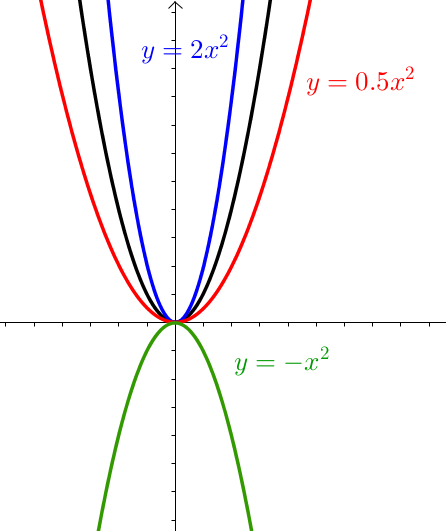
\includegraphics[width=4cm]{images/streckung.png}} & $a$ bewirkt& \gap{7.5} \\
			& $a>1$:  & \gap{7.5} \\
			& $0<a<1$: & \gap{7.5} \\
			& $a<0$: & \gap{7.5} \\
		\end{tabular}
	\end{table}
	\vspace*{2.5cm}
	%Verschiebung y-Richtung
\subsubsection*{$f(x)=x^2\mathbf{+v}$}
	\begin{table}[ht]
		\centering
		\begin{tabular}{cll}
			\multirow{3}{*}{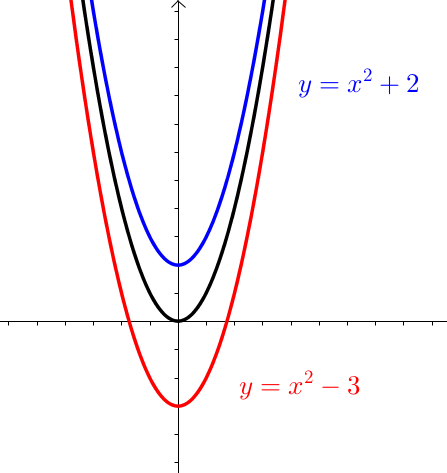
\includegraphics[width=4cm]{images/vertikaleverschiebung.png}} & $v$ bewirkt& \gap{7.5}\\
			& $v>0$:  & \gap{7.5}\\
			& $v<0$: & \gap{7.5}
		\end{tabular}
	\end{table}
	\vspace*{2.5cm}
	%Verschiebung x-Richtung
\subsubsection*{$f(x)= (x\mathbf{-u})^2$}
	\begin{table}[ht]
		\centering
		\begin{tabular}{cll}
			\multirow{3}{*}{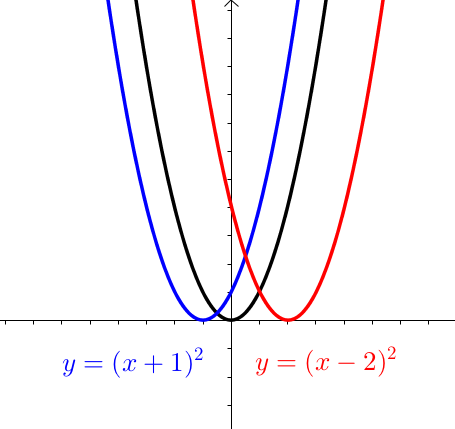
\includegraphics[width=4cm]{images/horizontaleverschiebung.png}} & $u$ bewirkt& \gap{7.5}\\
			& $u>0$:  & \gap{7.5}\\
			& $u<0$: & \gap{7.5}
		\end{tabular}
	\end{table}
	\endgroup
	\newpage
	\begin{aufgabe}
		Beschreibe in Worten, wie die Parabel aus der Normalparabel entstanden ist.
		\begin{enumcols}[2]
			\item $y=2x^2+4$
			\item $y=(x-3)^2+2$
			\item $y=\frac{1}{3}x^2-1$
			\item $y=-(x+2)^2$
		\end{enumcols}
	\end{aufgabe}
	\begin{aufgabe}
		Gebe für jede der folgenden Parabeln ohne zu rechnen oder zu zeichnen die Anzahl Nullstellen an.
		\begin{enumcols}[2]
			\item $y=x^2-3$
			\item $y=-(x+2)^2$
			\item $y=-x^2-5$
			\item $y=\frac{2}{3}(x-2)^2$
		\end{enumcols}
	\end{aufgabe}
	\begin{aufgabe}
		Zeichne die folgenden Funktionen (wenn möglich in verschiedenen Farben) in das Koordinatensystem ein.
		\begin{enumcols}[2]
			\item $y=x^2$
			\item $y=(x-3)^2$
			\item $y=-(x+1)^2+4$
			\item $y=2(x-1)^2+4$
		\end{enumcols}
		\begin{figure}[H]
			\centering
			\begin{tikzpicture}[cross/.style={draw, cross out, minimum size=2*(#1-1pt), inner sep=0pt, outer sep=0pt}, x=1cm, y=1cm,
				>=latex,   %Voreinstellung für Pfeilspitzen
				font= \footnotesize, scale=0.5]
				%Raster zeichnen
				\draw [color=gray!50]  [step=10mm] (-10.3,-10.3) grid (10.3,10.3);
				% Achsen zeichnen
				\draw[->,thick] (-10.3,0) -- (10.8,0) node[right, below] {\normalsize $x$};
				\draw[->,thick] (0,-10.3) -- (0,10.8) node[above, left] {\normalsize $y$};
				% Achsen beschriften
				\foreach \x in {-10,-8,...,-2,2,4,...,10} \draw (\x,-.1) -- (\x,.1) node[below=4pt] {$\x$};
				\foreach \y in {-10,-8,...,-2,2,4,...,10} \draw (-.1,\y) -- (.1,\y) node[left=4pt] {$\y$};
				% Besserer Ursprung
				\draw[color=black] (0pt,-14pt) node[right] {$0$};
				%Funktionen zeichnen:
				%\clip(-3.3,-5.3) rectangle (3.3,7.3); %Bildbereich
				%\draw[blue, smooth, domain=-9:9] plot (\x, {-1*pow(\x-3,2)+1}) node[yshift=13cm] {$$};
				%\draw[green, smooth, domain=-9:9] plot (\x, {2*pow(\x-3,2)-3}) node[] {$$};
				%\draw[red, smooth, domain=-9:9] plot (\x, {-0.4*pow(\x+3,2)+1}) node[right] {$$};
				%Beschriftung
				%\node[blue]  at (1,-5) {$p_2$};
			\end{tikzpicture}
		\end{figure}
	\end{aufgabe}



\newpage
\section{Scheitelpunktform}
\subsection{Von der Normalform zur Scheitelpunktform}
	\begin{align*}
		\mathbf{y=ax^2+bx+c \quad \longrightarrow \quad y=a(x-u)^2+v}
	\end{align*}
	Du hast im letzten Abschnitt gelernt, wie du den Graphen einer quadratische Funktion, die in der \textbf{Scheitelpunktsform} $y=a(x-u)^2+v$ gegeben ist, zeichnen kannst, und umgekehrt aus einem gegebenen Graphen die zugehörige quadratische Funktion findest. Wenn die Funktion in der \textbf{Normalform} $y=ax^2+bx+c$ gegeben ist, musst du sie zuerst in die Scheitelpunktsform bringen.
	\begin{aufgabe}
		Betrachte dazu den folgenden Lösungsweg. Notiere bei jeder Zeile, welche Umformungen vorgenommen wurde.
		\begin{align*}
			f:y&=2x^2+8x-3 &&\vert \\
			y+3&=2x^2+8x &&\vert \\
			\frac{y+3}{2}&=x^2+4x &&\vert \\
			\frac{y+3}{2}&=x^2+2\*2x &&\vert \\
			\frac{y+3}{2}+(2)^2&=x^2+2\*2x+(2)^2 &&\vert \\
			\frac{y+3}{2}+4&=(x+2)^2 &&\vert \\
			\frac{y}{2}+\frac{11}{2}&=(x+2)^2 &&\vert \\
			\frac{y}{2}&=(x+2)^2-\frac{11}{2} &&\vert \\
			f:y&=2\*(x+2)^2-11
		\end{align*}
		Um welches Verfahren handelt es sich hier? \gap{7}
	\end{aufgabe}
	Obwohl wir dieses Verfahren bereits bei den quadratischen Gleichungen sehr intensiv geübt haben. Hier nochmals eine weitere Aufgabe.
	\begin{aufgabe}
		Bringe die folgenden Funktionen in die Scheitelpunktform und zeichnen sie in verschiedenen Farben ins Koordinatensystem.
		\begin{enumcols}[2]
			\item $y=x^2-8x$
			\item $y=x^2+x$
			\item $y=2x^2-4x$
			\item $y=x^2-6x+11$
			\item $y=2x^2+8x-1$
			\item $y=-0.5x^2+6x-7$
		\end{enumcols}
		\begin{figure}[H]
			\centering
			\begin{tikzpicture}[cross/.style={draw, cross out, minimum size=2*(#1-1pt), inner sep=0pt, outer sep=0pt}, x=1cm, y=1cm,
				>=latex,   %Voreinstellung für Pfeilspitzen
				font= \footnotesize, scale=0.25]
				%Raster zeichnen
				\draw [color=gray!50]  [step=10mm] (-20.3,-20.3) grid (20.3,20.3);
				% Achsen zeichnen
				\draw[->,thick] (-20.3,0) -- (21.3,0) node[right, below] {\normalsize $x$};
				\draw[->,thick] (0,-20.3) -- (0,21.3) node[above, left] {\normalsize $y$};
				% Achsen beschriften
				\foreach \x in {-20,-15,-10,-5,5,10,15,20} \draw (\x,-.1) -- (\x,.1) node[below=4pt] {$\x$};
				\foreach \y in {-20,-15,-10,-5,5,10,15,20} \draw (-.1,\y) -- (.1,\y) node[left=4pt] {$\y$};
				% Besserer Ursprung
				\draw[color=black] (0pt,-20pt) node[right] {$0$};
				%Funktionen zeichnen:
				\clip(-20.3,-20.3) rectangle (20.8,20.8); %Bildbereich
				\draw[highdive,samples=100] plot (\x, {pow(\x,2)});
				%Beschriftung
				%\node[highdive]  at (5,18) {$p$};
			\end{tikzpicture}
		\end{figure}
	\end{aufgabe}
	Glücklicherweise kann dieser Prozess des quadratischen Ergänzens umgangen werden. Dazu nutzen wir die Symmetrie-Eigenschaften der Parabel aus. Der Scheitelpunkt $S(x_S,y_S)$ liegt exakt in der Mitte zwischen den beiden Nullstellen $x_1$ und $x_2$. Zusammen mit der Auflösungsformel für quadratische Gleichungen können wir die Koordinaten explizit berechnen:
	\begin{align*}
		x_S=\frac{1}{2}(x_1+x_2)&=\frac{1}{2}\left(\frac{-b+\sqrt{b^2-4ac}}{2a}+\frac{-b-\sqrt{b^2-4ac}}{2a}\right)\\
		&=\frac{1}{2}\left(\frac{-b+\sqrt{b^2-4ac}-b-\sqrt{b^2-4ac}}{2a}\right)\\
		&=\frac{-2b}{4a}=-\frac{b}{2a}
	\end{align*}
	\begin{satz}
		Ist eine quadratische Funktion in der Normalform $f:y=ax^2+bx+c$ gegeben, so besitzt der Scheitelpunkt die Koordinaten:
		\[S=\left(-\frac{b}{2a},-\frac{b^2-4ac}{4a}\right)\]
		Das heisst also, für die Parameter der Scheitelpunktform gilt: $\mathbf{u}=-\frac{b}{2a}$ und $\mathbf{v}=-\frac{b^2-4ac}{4a}$.
	\end{satz}
	\begin{aufgabe}
		Bestimme den Scheitelpunkt und die Nullstellen der folgenden beiden quadratischen Funktionen.
		\begin{enumcols}[2]
			\item $f:y=2x^2-5x+3$
			\item $g:y=-\frac{1}{5}(x+8)(x-2)$
		\end{enumcols}
	\end{aufgabe}
	\begin{aufgabe}
		\begin{minipage}{0.575\linewidth}
			Betrachte den folgenden Graphen und notiere die Funktionsgleichungen der abgebildeten Parabeln in Normalform.\vspace{5pt}\newline\karos{4.5}
		\end{minipage}
		\hfill
		\begin{minipage}{0.4\linewidth}
			\begin{tikzpicture}[cross/.style={draw, cross out, minimum size=2*(#1-1pt), inner sep=0pt, outer sep=0pt}, x=1cm, y=1cm,
				>=latex,   %Voreinstellung für Pfeilspitzen
				font= \footnotesize, scale=0.5]
				%Raster zeichnen
				\draw [color=gray!50]  [step=10mm] (-5.3,-5.3) grid (5.3,5.3);
				% Achsen zeichnen
				\draw[->,thick] (-5.3,0) -- (5.8,0) node[right, below] {\normalsize $x$};
				\draw[->,thick] (0,-5.3) -- (0,5.8) node[above, left] {\normalsize $y$};
				% Achsen beschriften
				\foreach \x in {-5,-4,...,-1,1,2,...,5} \draw (\x,-.1) -- (\x,.1) node[below=4pt] {$\x$};
				\foreach \y in {-5,-4,...,-1,1,2,...,5} \draw (-.1,\y) -- (.1,\y) node[left=4pt] {$\y$};
				% Besserer Ursprung
				\draw[color=black] (0pt,-20pt) node[right] {$0$};
				%Funktionen zeichnen:
				\clip(-5.3,-5.3) rectangle (5.5,5.5); %Bildbereich
				\draw[highdive,samples=100] plot (\x, {2*pow(\x-3,2)-2});
				\draw[forestgreen,samples=100] plot (\x, {-1*pow(\x+2,2)+4});
				\draw[plotblue,samples=100] plot (\x, {pow(\x-2,2)+2});
				\draw[red,samples=100] plot (\x, {-0.5*pow(\x,2)+1});
				%Beschriftung
				%\node[highdive]  at (4.5,1.5) {$f$};
			\end{tikzpicture}
		\end{minipage}
	\end{aufgabe}



\newpage
\section{Typische Fragestellungen bei quadratischen Funktionen}
	Typische Fragen beim Bearbeiten von Problemen mit quadratischen Funktionen sind unter anderem diese:
	\begin{enumerate}
		\item Wo schneidet der Graph die $x$-Achse?
		\item Wo ist der höchste/niedrigste Punkt des Graphen?
		\item Welchen $y$-Wert erhält man für einen bestimmten $x$-Wert?
		\item Welchen $x$-Wert erhält man für einen bestimmten $y$-Wert?
	\end{enumerate}
	Um diese Fragen an einem konkreten Beispiel zu beantworten, betrachten wir das folgende Beispiel:

\subsection*{Beispiel: Rakete}
	Nach dem Abschuss einer Rakete kann man jedem Zeitpunkt $t$ die aktuelle Höhe $h(t)$ der Rakete zuordnen. Man kann diese Zuordnung bei allen Raketen gut mit einer quadratischen Funktion modellieren.\newline
	\textbf{Funktionsgleichung:} \[h(t)=-5t^2+45t+50\]
	Vervollständige die Wertetabelle und zeichne den Graphen:
	\begingroup
	\renewcommand{\arraystretch}{1.5}
	\begin{table}[ht]
		\centering
		\begin{tabular}{|p{2cm}|p{0.6cm}|p{0.6cm}|p{0.6cm}|p{0.6cm}|p{0.6cm}|p{0.6cm}|p{0.6cm}|p{0.6cm}|p{0.6cm}|p{0.6cm}|}\hline
			$t$ (in sec) & $1$ & $2$ & $3$ & $4$ & $5$ & $6$ & $7$ & $8$ & $9$ & $10$ \\ \hline
			$h(t)$ (in m) & $90$ & $120$ & & & & & & & & \\ \hline
		\end{tabular}
	\end{table}
	\endgroup
	\begin{figure}[ht]
		\centering
		\begin{tikzpicture}[cross/.style={draw, cross out, minimum size=2*(#1-1pt), inner sep=0pt, outer sep=0pt}, x=1cm, y=1mm,
			>=latex,   %Voreinstellung für Pfeilspitzen
			font=\footnotesize, scale=0.5]
			%Raster zeichnen
			\draw [color=gray!50]  [step=10mm] (-4.3,-23) grid (12.3,143);
			% Achsen zeichnen
			\draw[->,thick] (-4.3,0) -- (12.8,0) node[right, below] {\normalsize $x$};
			\draw[->,thick] (0,-23) -- (0,148) node[above, left] {\normalsize $y$};
			% Achsen beschriften
			\foreach \x in {-4,-2,2,4,...,12} \draw (\x,-1) -- (\x,1) node[below=4pt] {$\x$};
			\foreach \y in {-20,20,40,...,140} \draw (-.1,\y) -- (.1,\y) node[left=4pt] {$\y$};
			% Besserer Ursprung
			\draw[color=black] (0pt,-20pt) node[right] {$0$};
			%Funktionen zeichnen:
			\clip(-2.3,-23) rectangle (12.3,143); %Bildbereich
			%\draw[highdive,samples=100] plot (\x, {pow(\x,2)});
			%Beschriftung
			%\node[highdive]  at (5,18) {$p$};
		\end{tikzpicture}
	\end{figure}
	\begin{aufgabe}
		Beantworte die folgenden Fragen und zeichne die Punkte im Graphen ein:
		\begin{enumerate}[label=\alph*)]
			\item Welche grösste Höhe erreicht die Rakete nach welcher Flugzeit?
			\item Wann trifft die Rakete auf dem Boden auf?
			\item Nach welcher Zeit hat die Rakete eine Höhe von $90$m?
			\item Wie hoch fliegt die Rakete nach $3$s?
		\end{enumerate}
		Ordne die Fragen $a$ - $d$ den Buchstaben $1-4$ zu.
	\end{aufgabe}
	\begin{aufgabe}[Weitere Beispiele]
		\begin{enumerate}
			\item BlaBlaBla
			\item BleBleBle
			\item BloBloBlo
			\item BluBluBlu
		\end{enumerate}
	\end{aufgabe}


\newpage
\section{Schnittpunktprobleme}
\subsection{Schnittpunkte von Parabel mit Gerade}
	Werden mehrere Graphen in einem Koordinatensystem dargestellt, stellt sich sehr häufig die Frage nach gemeinsamen Punkten. Wie möchten dies für die Kombination einer Parabel und einer Gerade betrachten.
	\begin{align*}
		\text{Parabel:}\qquad p:y&=ax^2+bx+c\\
		\text{Gerade:}\qquad g:y&=m\*x+q
	\end{align*}
	Die gemeinsamen Punkte oder eben Schnittpunkte erfüllen beide Funktionsgleichungen. Das heisst, wir können die rechte Seite der obigen Gleichungen gleichsetzen.
	\begin{align*}
		p(x)&=g(x)\\
		ax^2+bx+c&=mx+q &&\vert -mx-q\\
		ax^2+(b-m)\*x+(c-q)&=0
	\end{align*}
	Die $x-$Koordinaten der Schnittpunkte sind also die Lösungen der obigen quadratischen Gleichung. Das wir haben auch hier drei verschiedene Szenarien, abhängig wie viele Lösungen die Gleichung besitzt.\vspace{22pt}\newline
	\begin{minipage}{0.3\linewidth}
		\centering
		Gerade \textbf{schneidet} Parabel
		\begin{tikzpicture}[cross/.style={draw, cross out, minimum size=2*(#1-1pt), inner sep=0pt, outer sep=0pt}, x=1cm, y=1cm,
			>=latex,   %Voreinstellung für Pfeilspitzen
			font=\footnotesize, scale=0.4]
			%Raster zeichnen
			\draw [color=gray!50]  [step=10mm] (-3.3,-8.3) grid (7.3,8.3);
			% Achsen zeichnen
			\draw[->,thick] (-3.3,0) -- (7.8,0) node[right, below] {\normalsize $x$};
			\draw[->,thick] (0,-8.3) -- (0,8.8) node[above, left] {\normalsize $y$};
			% Achsen beschriften
			\foreach \x in {-3,-2,-1,1,2,...,7} \draw (\x,-.1) -- (\x,.1) node[below=4pt] {$\x$};
			\foreach \y in {-8,-6,...,-2,2,4,...,8} \draw (-.2,\y) -- (.2,\y) node[left=4pt] {$\y$};
			% Besserer Ursprung
			\draw[color=black] (0pt,-10pt) node[right] {$0$};
			%Funktionen zeichnen:
			\clip(-3.3,-8.3) rectangle (7.3,8.3); %Bildbereich
			\draw[highdive,domain=-2:7,samples=100] plot (\x, {-pow(\x,2)+5*\x});
			\draw[highdive,domain=-3.3:7.3,samples=100] plot (\x,{-2/3*\x+5});
			%Beschriftung
			%\node[highdive]  at (5,18) {$p$};
		\end{tikzpicture}
		Diskriminante $\mathbf{D>0}$
	\end{minipage}
	\hfill
	\begin{minipage}{0.3\linewidth}
		\centering
		Gerade \textbf{berührt} Parabel
		\begin{tikzpicture}[cross/.style={draw, cross out, minimum size=2*(#1-1pt), inner sep=0pt, outer sep=0pt}, x=1cm, y=1cm,
			>=latex,   %Voreinstellung für Pfeilspitzen
			font=\footnotesize, scale=0.4]
			%Raster zeichnen
			\draw [color=gray!50]  [step=10mm] (-9.3,-8.3) grid (1.3,8.3);
			% Achsen zeichnen
			\draw[->,thick] (-9.3,0) -- (1.8,0) node[right, below] {\normalsize $x$};
			\draw[->,thick] (0,-8.3) -- (0,8.8) node[above, left] {\normalsize $y$};
			% Achsen beschriften
			\foreach \x in {-9,-8,...,-1,1} \draw (\x,-.1) -- (\x,.1) node[below=4pt] {$\x$};
			\foreach \y in {-8,-6,...,-2,2,4,...,8} \draw (-.2,\y) -- (.2,\y) node[left=4pt] {$\y$};
			% Besserer Ursprung
			\draw[color=black] (0pt,-10pt) node[right] {$0$};
			%Funktionen zeichnen:
			\clip(-9.3,-8.3) rectangle (1.3,8.3); %Bildbereich
			\draw[highdive,domain=-9.3:1.3,samples=100] plot (\x, {-0.5*pow(\x,2)-4*\x-3});
			\draw[highdive,domain=-9.3:1.3,samples=100] plot (\x,{2*\x+15});
			%Beschriftung
			%\node[highdive]  at (5,18) {$p$};
		\end{tikzpicture}
		Diskriminante $\mathbf{D=0}$
	\end{minipage}
	\hfill
	\begin{minipage}{0.3\linewidth}
		\centering
		Gerade \textbf{meidet} Parabel
		\begin{tikzpicture}[cross/.style={draw, cross out, minimum size=2*(#1-1pt), inner sep=0pt, outer sep=0pt}, x=1cm, y=1cm,
			>=latex,   %Voreinstellung für Pfeilspitzen
			font=\footnotesize, scale=0.4]
			%Raster zeichnen
			\draw [color=gray!50]  [step=10mm] (-3.3,-8.3) grid (7.3,8.3);
			% Achsen zeichnen
			\draw[->,thick] (-3.3,0) -- (7.8,0) node[right, below] {\normalsize $x$};
			\draw[->,thick] (0,-8.3) -- (0,8.8) node[above, left] {\normalsize $y$};
			% Achsen beschriften
			\foreach \x in {-3,-2,-1,1,2,...,7} \draw (\x,-.1) -- (\x,.1) node[below=4pt] {$\x$};
			\foreach \y in {-8,-6,...,-2,2,4,...,8} \draw (-.2,\y) -- (.2,\y) node[left=4pt] {$\y$};
			% Besserer Ursprung
			\draw[color=black] (0pt,-10pt) node[right] {$0$};
			%Funktionen zeichnen:
			\clip(-3.3,-8.3) rectangle (7.3,8.3); %Bildbereich
			\draw[highdive,domain=-3.3:7.3,samples=100] plot (\x, {3*pow(\x,2)-6*\x+4});
			\draw[highdive,domain=-3.3:7.3,samples=100] plot (\x,{\x-5});
			%Beschriftung
			%\node[highdive]  at (5,18) {$p$};
		\end{tikzpicture}
		Diskriminante $\mathbf{D<0}$
	\end{minipage}
	\begin{aufgabe}
		Bestimme die Schnittpunkte der folgenden Parabel mit der Gerade.
		\begin{enumerate}[label=\alph*)]
			\item $\displaystyle p:y=2x^2-3x+4 \text{ und } g:y=-2x+6$
			\item $\displaystyle p:y=4x^2+12x-5\text{ und } g:y=2x-5$
		\end{enumerate}
	\end{aufgabe}
	\begin{aufgabe}
		Gegeben sind die folgenden Funktionen: \[p:y=-\frac{1}{2}x^2+3x,\qquad g:y=2x+\frac{1}{2},\qquad h:y=-4x+\frac{49}{2}\]
		\begin{enumerate}[label=\alph*)]
			\item Zeige, dass die beiden Geraden $g$ und $h$ die Parabel $p$ in einem Punkt berühren.
			\item Gib die Koordinaten des Berührungspunktes an.
		\end{enumerate}
	\end{aufgabe}
\subsection{Schnittpunkte von zwei Parabeln}
	Um den Schnittpunkt zweier Parabeln zu bestimmen, gehen wir genau gleich vor wie bei Parabel und Gerade. Das heisst, auch hier setzen wir die beiden Funktionsgleichungen gleich und lösen nach der Variabel $x$ auf.
	\begin{beispiel}
		Berechne die Schnittpunkte der Normalparabel mit der Parabel $f:y=-\frac{1}{2}x^2+3x+\frac{9}{2}$.
		\begin{minipage}{0.45\linewidth}
			\centering
			\begin{tikzpicture}[cross/.style={draw, cross out, minimum size=2*(#1-1pt), inner sep=0pt, outer sep=0pt}, x=1cm, y=1cm,
				>=latex,   %Voreinstellung für Pfeilspitzen
				font=\footnotesize, scale=0.4]
				%Raster zeichnen
				\draw [color=gray!50]  [step=10mm] (-6.3,-6.3) grid (11.3,11.3);
				% Achsen zeichnen
				\draw[->,thick] (-6.3,0) -- (11.8,0) node[right, below] {\normalsize $x$};
				\draw[->,thick] (0,-6.3) -- (0,11.8) node[above, left] {\normalsize $y$};
				% Achsen beschriften
				\foreach \x in {-5,5,10} \draw (\x,-.1) -- (\x,.1) node[below=4pt] {$\x$};
				\foreach \y in {-5,5,10} \draw (-.1,\y) -- (.1,\y) node[left=4pt] {$\y$};
				% Besserer Ursprung
				\draw[color=black] (0pt,-10pt) node[right] {$0$};
				%Funktionen zeichnen:
				\clip(-6.3,-6.3) rectangle (11.3,11.3); %Bildbereich
				\draw[highdive,domain=-5:10,samples=100] plot (\x, {-0.5*pow(\x,2)+3*\x+4.5});
				\draw[highdive,samples=100] plot (\x,{pow(\x,2)});
				%Beschriftung
				%\node[highdive]  at (5,18) {$p$};
			\end{tikzpicture}
		\end{minipage}
		\hfill
		\begin{minipage}{0.5\linewidth}
			\vspace{5cm}
		\end{minipage}\vspace{3cm}
	\end{beispiel}

	\begin{aufgabe}
		Berechne die Schnittpunkte der beiden Parabeln.
		\begin{enumerate}[label=\alph*)]
			\item $p_1:y=x^2-7$ und $p_2:y=\frac{1}{3}x^2-1$
			\item $p_1:y=\frac{1}{2}x^2-5x+\frac{19}{2}$ und $p_2:y=-\frac{1}{6}x^2+\frac{1}{3}x+\frac{29}{6}$
		\end{enumerate}
	\end{aufgabe}


\newpage
\section{Funktionsgleichung bestimmen}
	Für eine lineare Funktion der Form $y=m\cdot x+q$ haben wir bereits ein Verfahren kennengelernt, wie man die Funktionsgleichung anhand gegebener Punkte bestimmen kann. Dort haben wir festgestellt, dass zwei Punkte für eine eindeutige Bestimmung der zwei Parameter reichen. Analog gilt für die quadratischen Funktionen:\vspace{11pt}\newline
	\fbox{\textbf{Ansatz: $f(x)=a\cdot x^2+b\cdot x+c$}}\vspace{11pt}\newline
	Wie wir in der obigen Gleichung sehen, haben wir nun drei Unbekannte $a$, $b$ und $c$. Das heisst, wir benötigen mindestens drei Punkte, um die Funktionsgleichung eindeutig zu bestimmen.
	\begin{beispiel}
		Bestimme die Funktionsgleichung der Parabel, die durch die Punkte $P=(1,0)$, $Q=(0,-1)$ und $R=(-1,-6)$ verläuft.
	\end{beispiel}
	\subsection*{Von Hand}
	\vspace{8cm}
	\subsection*{Mit Taschenrechner}
	Menu $->$ 2 $->$ 3 $->$ 1
	\newpage
	\begin{aufgabe}
		Finde die Funktionsgleichung der Parabel, die durch die gegebenen Punkte verläuft.
		\begin{enumcols}[2]
			\item blablabla
			\item blublublu
		\end{enumcols}
	\end{aufgabe}



\newpage
\section{Modellieren}



\newpage
\section{Extremwertaufgaben}


\newpage
\subsection*{History}
\begin{table}[H]
	\centering
	\begin{tabular}{|p{13mm}|p{20mm}|p{30mm}|p{70mm}|}\hline
		%\multicolumn{4}{|l|}{History}\\\hline
		Version & Datum & Person & Bemerkung \\\hline
		$0.1$ & 22.12.2023 & Jonas Guler & Kapitel erstellt \\\hline
		$0.2$ & 09.12.2024 & Jonas Guler & Korrekturen \\\hline
		& ToDo & Jonas Guler & Funktionsgleichung bestimmen, Modellieren und Extremwertaufgaben fehlen \\\hline
	\end{tabular}
\end{table}



\end{document}